\documentclass[portuguese,brazil]{beamer}
\usepackage[utf8]{inputenc}   %% UTF-8 Encoding
\usepackage{graphicx} %% include graphics, preferrably pdf

\usetheme{Malmoe}
\usecolortheme{git}
\usefonttheme{progressbar}
%\useoutertheme{progressbar}
\useinnertheme{progressbar}

% Remove o headline do tema Malmoe
\setbeamertemplate{headline}{\vskip .3cm}

\progressbaroptions{headline=sections,frametitle=picture-subsection}

% Número da página no rodapé
\newcommand*\oldmacro{}
\let\oldmacro\insertshortauthor% save previous definition
\renewcommand*\insertshortauthor{%
  \leftskip=.3cm% before the author could be a plus1fill ...
    \insertframenumber\,/\,\inserttotalframenumber\hfill\oldmacro}

% Macro para facilitar a criação de slides com uma única frase
\newcommand\singlephrase[1]{
  \begin{center}
    \huge #1
  \end{center}
}

\newcommand\img[1]{
  \begin{center}
    \includegraphics{#1}
  \end{center}
}

\newcommand\sectiontoc{
  \begin{frame}
    \tableofcontents[currentsection]
  \end{frame}
}

\title[Controle de Versão com git]{Controle de Versão com git}
\author{Felipe Oliveira Carvalho}
\institute{Universidade Federal de Sergipe}
\date{6 de Outubro, 2011}


\begin{document}

\begin{frame}
  \titlepage
\end{frame}

\begin{frame}
  \tableofcontents
\end{frame}

\section{Introdução}

\subsection{O que é controle de versão?}

\begin{frame}{O que é controle de versão?}
Controle de versão é um sistema que grava as mudanças feitas em um conjunto de
arquivos ao longo do tempo de uma forma que você possa restaurar e comparar versões
específicas depois.
\pause

Tipos de controle de versão:
\begin{itemize}
  \item Controle de versão local
  \item Controle de versão centralizado
  \item Controle de versão distribuído
\end{itemize}
\end{frame}

\begin{frame}{Controle de versão local}
  \img{images/localvcs.png}
\end{frame}

\begin{frame}{Controle de versão centralizado}
  \img{images/centralvcs.png}
\end{frame}

\begin{frame}{Controle de versão distribuído}
\begin{center}
  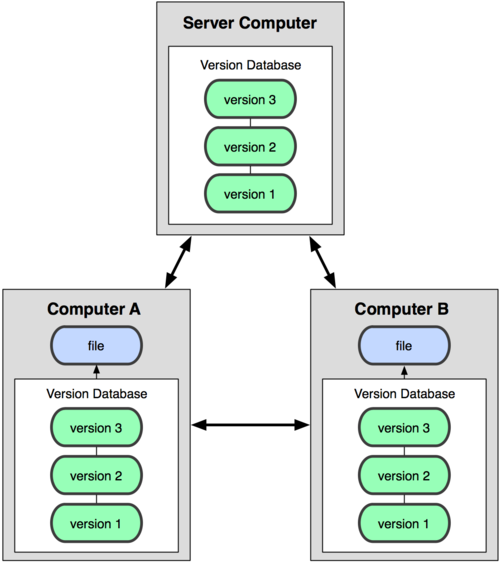
\includegraphics[scale=.65]{images/distributedvcs.png}
\end{center}
\end{frame}

\subsection{O que é git?}

\begin{frame}{O que é git?}
\singlephrase{\textbf{Git} é um sistema de controle de versão
\textbf{distribuído} projetado para ser \textbf{eficiente}.}
\end{frame}

\begin{frame}{Breve história}
\begin{itemize}
\item Criado por Linus Torvalds em 2005
\item Para ser usado no desenvolvimento do Linux kernel
\item Metas dos projeto:
\begin{itemize}
\item Velocidade
\item Design simples
\item Permitir desenvolvimento não-linear (milhares de branches)
\item Capaz de manipular projetos grandes como o Linux kernel de maneira eficiente
\end{itemize}
\end{itemize}
\end{frame}

\section{Introdução ao git}

\sectiontoc

\subsection{Primeiros passos}

\begin{frame}{Instalação}
\begin{center}
  http://git-scm.com
  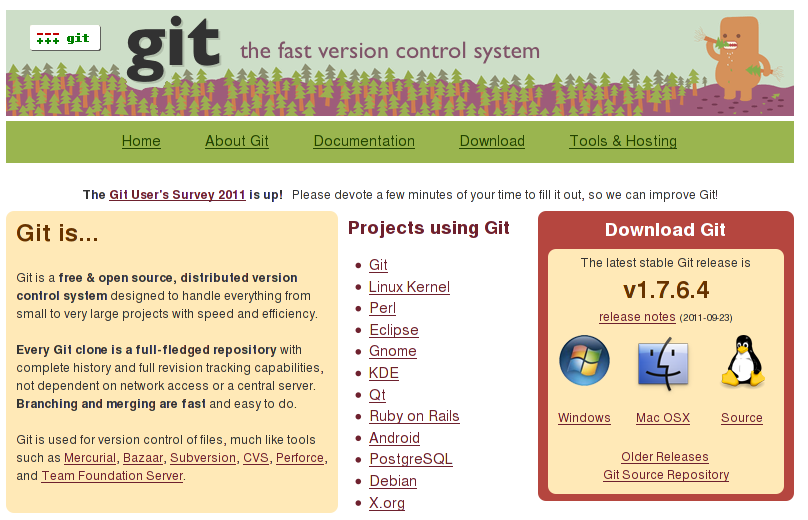
\includegraphics[scale=.38]{images/gitscm.png}
\end{center}
\end{frame}

\begin{frame}[fragile]{Configurando}
\begin{verbatim}
$ git config --global user.name "Felipe O. Carvalho"
$ git config --global user.email "felipekde@gmail.com"
\end{verbatim}
\end{frame}

\subsection{Repositórios}

\begin{frame}[fragile]{Criando um repositório}
\begin{center}
\texttt{git init}
\end{center}
\begin{verbatim}
$ mkdir hello_git
$ cd hello_git/
$ git init
Initialized empty Git repository in /home/felipe/hello_git/.git/
$ ls -a
.  ..  .git
\end{verbatim}
\end{frame}

\begin{frame}[fragile]{Primeiro commit}
\begin{center}
\texttt{git add}\\
\texttt{git commit}
\end{center}
\begin{verbatim}
$ touch hello_world.py
$ git add hello_world.py
$ git commit -m "Primeiro commit"
\end{verbatim}
\end{frame}

\begin{frame}[fragile]{Primeiro commit}
\small{
\begin{verbatim}
$ git show
\end{verbatim}
\pause
\begin{verbatim}
commit 9b302737d41712809ca455b1d522c334793ef001
Author: Felipe Oliveira Carvalho <felipekde@gmail.com>
Date:   Sun Oct 2 15:45:23 2011 -0300

    Primeiro commit

    diff --git a/hello_world.py b/hello_world.py
    new file mode 100644
    index 0000000..e69de29
\end{verbatim}
}
\end{frame}

\begin{frame}[fragile]{Clonando um Repositório}
\vskip 0pt 
\begin{center}
\texttt{git clone}
\end{center}
\begin{verbatim}
$ git clone git://github.com/schacon/ticgit.git
\end{verbatim}
\pause
\tiny{
\begin{verbatim}
Cloning into ticgit...
remote: Counting objects: 1857, done.
remote: Compressing objects: 100% (826/826), done.
remote: Total 1857 (delta 969), reused 1796 (delta 931)
Receiving objects: 100% (1857/1857), 269.46 KiB | 143 KiB/s, done.
Resolving deltas: 100% (969/969), done.
\end{verbatim}
}
\pause
\small{
\begin{verbatim}
$ cd ticgit
\end{verbatim}
\pause
\begin{verbatim}
$ ls
\end{verbatim}
}
\pause
\tiny{
\begin{verbatim}
bin  examples  lib  LICENSE_GPL  LICENSE_MIT note  Rakefile
README.mkd  spec ticgit-ng.gemspec  TODO
\end{verbatim}
}
\end{frame}

\begin{frame}{gitk}
\begin{center}
  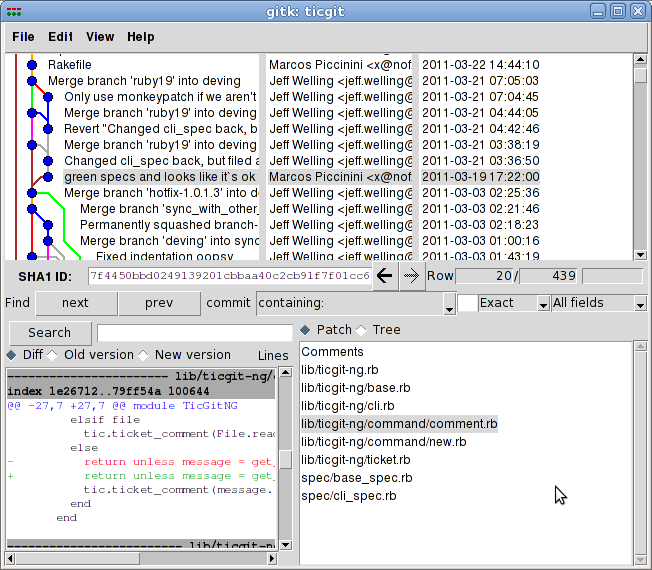
\includegraphics[scale=.38]{images/gitkticgit.png}
\end{center}
\end{frame}

\subsection{Workflow básico}

\begin{frame}{Workflow básico}
  \begin{itemize}
    \item Editar arquivos
    \pause
    -- \textbf{Eclipse, Visual Studio, Notepad++, emacs, vim... Photoshop...}
    \pause
    \item Adicionar as mudanças ao \textit{index} (também conhecido como
      \textit{staging area}
    \pause
    -- \textbf{git add, git rm, git reset...}
    \pause
    \item Revisar as mudanças
    -- \textbf{git status, git diff...}
    \pause
    \item Fazer o \textit{commit} das mudanças
    -- \textbf{git commit -m "Mensagem"}
  \end{itemize}
\end{frame}

\begin{frame}{Os três passos}
  \img{images/three.png}
\end{frame}

\begin{frame}[fragile]{Os três passos}
\small{
\begin{verbatim}
$ vim hello_world.py
\end{verbatim}
\pause
\begin{verbatim}
$ cat hello_world.py
print "Hell World!"
\end{verbatim}
\pause
\begin{verbatim}
$ git status
\end{verbatim}
\pause
\tiny{
\begin{verbatim}
# On branch master
# Changes not staged for commit:
#   (use "git add <file>..." to update what will be committed)
#   (use "git checkout -- <file>..." to discard changes in working directory)
#
#       modified:   hello_world.py
#
no changes added to commit (use "git add" and/or "git commit -a")
\end{verbatim}
}
}
\end{frame}

\begin{frame}{Os três passos}
\singlephrase{Você \textbf{tem} que adicionar o arquivo ao \textit{index} \textbf{depois}
de editá-lo e/ou criá-lo.}
\end{frame}

\begin{frame}{Os três passos}
  \img{images/staginandcommit.pdf}
\end{frame}

\begin{frame}[fragile]{Os três passos}
\small{
\begin{verbatim}
$ git add hello_world.py
\end{verbatim}
\pause
\begin{verbatim}
$ git status
# On branch master
# Changes to be committed:
#   (use "git reset HEAD <file>..." to unstage)
#
#       modified:   hello_world.py
#
\end{verbatim}
\pause
\begin{verbatim}
$ git commit -m "Hello World em Python"
\end{verbatim}
\pause
\begin{verbatim}
[master e3d5175] Hello World em Python
 1 files changed, 1 insertions(+), 0 deletions(-)
\end{verbatim}
\pause
\begin{verbatim}
$ git status
# On branch master
nothing to commit (working directory clean)
\end{verbatim}
}
\end{frame}

\begin{frame}[fragile]{Os três passos}
\small{
\begin{verbatim}
$ git log
commit e3d5175ca59febe510b1e0689040d2702b08c7ee
Author: Felipe Oliveira Carvalho <felipekde@gmail.com>
Date:   Sun Oct 2 17:36:41 2011 -0300

    Hello World em Python

commit 9b302737d41712809ca455b1d522c334793ef001
Author: Felipe Oliveira Carvalho <felipekde@gmail.com>
Date:   Sun Oct 2 15:45:23 2011 -0300

    Primeiro commit

\end{verbatim}
}
\end{frame}

\begin{frame}{Comandos vistos até agora}
  \begin{center}
    \begin{tabular}{l   l}
      \texttt{git config} & \textbf{Utilitário de configuração} \\
      \pause \\
      \texttt{git init} & \textbf{Cria um novo repositório} \\
      \texttt{git clone} & \textbf{Clona um repositório existente} \\
      \pause \\
      \texttt{git status} & \textbf{Mostra o estado do diretório de trabalho e index} \\
      \pause \\
      \texttt{git add} & \textbf{Adiciona arquivos ao index} \\
      \texttt{git commit} & \textbf{Faz o commit das mudanças no index} \\
      \texttt{git show} & \textbf{Mostra detalhes do último commit} \\
      \pause \\
      \texttt{git log} & \textbf{Lista os commits}
    \end{tabular}
  \end{center}
\end{frame}

\begin{frame}{Untracked, Unmodified, Modified e Staged}
  \img{images/filelifecycle.png}
\end{frame}

\begin{frame}[fragile]{Untracked, Unmodified, Modified e Staged}
\begin{verbatim}
$ git status
# On branch master
nothing to commit (working directory clean)
\end{verbatim}
\pause
\begin{verbatim}
$ vim README
\end{verbatim}
\pause
\textbf{Untracked}
\begin{verbatim}
$ git status
# On branch master
# Untracked files:
#   (use "git add <file>..." to include in what will be committed)
#
#       README
nothing added to commit but untracked files present (use "git add" to track)
\end{verbatim}
\end{frame}

\begin{frame}[fragile]{Untracked, Unmodified, Modified e Staged}
\begin{verbatim}
$ git add README
\end{verbatim}
\pause
\textbf{Staged}
\begin{verbatim}
$ git status
# On branch master
# Changes to be committed:
#   (use "git reset HEAD <file>..." to unstage)
#
#       new file:   README
#
\end{verbatim}
\end{frame}

\begin{frame}[fragile]{Untracked, Unmodified, Modified e Staged}
\begin{verbatim}
$ vim hello_git.py
\end{verbatim}
\pause
\textbf{Staged, Modified}
\tiny{
\begin{verbatim}
$ git status
# On branch master
# Changes to be committed:
#   (use "git reset HEAD <file>..." to unstage)
#
#       new file:   README
#
# Changes not staged for commit:
#   (use "git add <file>..." to update what will be committed)
#   (use "git checkout -- <file>..." to discard changes in working directory)
#
#       modified:   hello_world.py
#
\end{verbatim}
}
\end{frame}

\begin{frame}[fragile]{Untracked, Unmodified, Modified e Staged}
\begin{verbatim}
$ git add hello_world.py
\end{verbatim}
\pause
\textbf{Staged}
\begin{verbatim}
$ git status
# On branch master
# Changes to be committed:
#   (use "git reset HEAD <file>..." to unstage)
#
#       new file:   README
#       modified:   hello_world.py
#
\end{verbatim}
\end{frame}

\begin{frame}[fragile]{Untracked, Unmodified, Modified e Staged}
\begin{verbatim}
$ git commit -m "README e mudanças no Hello World"
[master 2b32cb9] README e mudanças no Hello World
 1 files changed, 1 insertions(+), 1 deletions(-)
 create mode 100644 README
\end{verbatim}
\pause
\textbf{Unmodified}
\begin{verbatim}
$ git status
# On branch master
nothing to commit (working directory clean)
\end{verbatim}
\end{frame}

\begin{frame}[fragile]{Visualizando modificações}
\begin{verbatim}
$ vim hello_world.py
\end{verbatim}
\pause
\begin{verbatim}
$ git status
[...]
$ git diff
[...]
$ git add hello_world.py
$ git status
[...]
$ git diff --staged
[...]
\end{verbatim}
\end{frame}

\begin{frame}[fragile]{Removendo arquivos}
\begin{verbatim}
$ rm README
\end{verbatim}
\pause
\begin{verbatim}
$ git status
# On branch master
# Changes not staged for commit:
#   (use "git add/rm <file>..." to update what will be committed)
#   (use "git checkout -- <file>..." to discard changes in working directory)
#
#       deleted:    README
#
no changes added to commit (use "git add" and/or "git commit -a")
\end{verbatim}
\end{frame}

\begin{frame}[fragile]{Removendo arquivos}
\begin{verbatim}
$ git rm README
rm 'README'
\end{verbatim}
\pause
\begin{verbatim}
$ git status
# On branch master
# Changes to be committed:
#   (use "git reset HEAD <file>..." to unstage)
#
#       deleted:    README
#
\end{verbatim}
\pause
\begin{verbatim}
$ git commit -m "Removi o README"
[master b09a767] Removi o README
 0 files changed, 0 insertions(+), 0 deletions(-)
 delete mode 100644 README
\end{verbatim}
\end{frame}

\subsection{Obtendo ajuda}

\begin{frame}[fragile]{Obtendo ajuda}
\begin{verbatim}
$ git help <verb>
$ git <verb> --help
$ man git-<verb>
$ git <verb> -h
\end{verbatim}
\tiny{
\begin{verbatim}
$ git commit -h
usage: git commit [options] [--] <filepattern>...

    -q, --quiet           suppress summary after successful commit
    -v, --verbose         show diff in commit message template

Commit message options
    -F, --file <file>     read message from file
    --author <author>     override author for commit
    --date <date>         override date for commit
    -m, --message <message>
                          commit message
    -c, --reedit-message <commit>
                          reuse and edit message from specified commit
    -C, --reuse-message <commit>
                          reuse message from specified commit
    --fixup <commit>      use autosquash formatted message to fixup specified commit
    --squash <commit>     use autosquash formatted message to squash specified commit
    --reset-author        the commit is authored by me now (used with -C-c/--amend)
    -s, --signoff         add Signed-off-by:
    -t, --template <file>
                          use specified template file
    -e, --edit            force edit of commit

...
\end{verbatim}
}
\end{frame}

\subsection{Visualizando o histórico do repositório}

\begin{frame}[fragile]{git log}
\tiny{
\begin{verbatim}
$ git log
commit b09a76779af9257ccd69c1fc5aac3e1dd0d03693
Author: Felipe Oliveira Carvalho <felipekde@gmail.com>
Date:   Sun Oct 2 22:41:32 2011 -0300

    Removi o README

commit 2b32cb93b49dbd87b2387f21ee3b945b4c822fbf
Author: Felipe Oliveira Carvalho <felipekde@gmail.com>
Date:   Sun Oct 2 22:25:23 2011 -0300

    README e mudanças no Hello World

commit e3d5175ca59febe510b1e0689040d2702b08c7ee
Author: Felipe Oliveira Carvalho <felipekde@gmail.com>
Date:   Sun Oct 2 17:36:41 2011 -0300

    Hello World em Python

commit 9b302737d41712809ca455b1d522c334793ef001
Author: Felipe Oliveira Carvalho <felipekde@gmail.com>
Date:   Sun Oct 2 15:45:23 2011 -0300

    Primeiro commit
\end{verbatim}
}
\end{frame}

\begin{frame}[fragile]{Visualizando um commit}
\begin{verbatim}
$ git show 2b32cb93
commit 2b32cb93b49dbd87b2387f21ee3b945b4c822fbf
Author: Felipe Oliveira Carvalho <felipekde@gmail.com>
Date:   Sun Oct 2 22:25:23 2011 -0300

    README e mudanças no Hello World

diff --git a/README b/README
new file mode 100644
index 0000000..e69de29
diff --git a/hello_world.py b/hello_world.py
index 088ea5c..ffee107 100644
--- a/hello_world.py
+++ b/hello_world.py
@@ -1 +1 @@
-print "Hell World!"
+print "Alô mundo!"
\end{verbatim}
\end{frame}

\begin{frame}{gitk}
\texttt{\$ gitk \&}
\begin{center}
  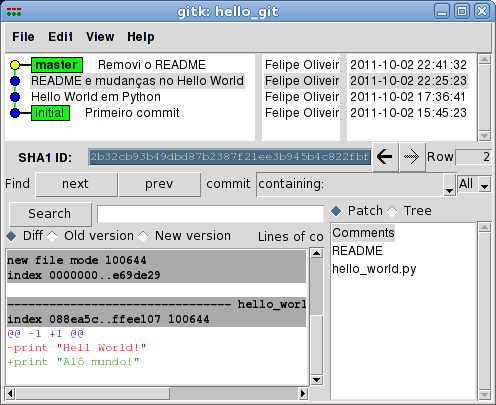
\includegraphics[scale=0.45]{images/gitkhellogit.png}
\end{center}
\end{frame}

\section{Branching e Merging}

\sectiontoc

\subsection{Armazenamento de commits}

\begin{frame}{Armazenamento de commits}
  \img{images/commitstore.png}
\end{frame}

\subsection{Branches}

\begin{frame}{Branches}
  \img{images/masterbranch.png}
\end{frame}

\begin{frame}{Criando um novo branch -- branching}
  \texttt{\$ git branch testing}
  \img{images/testingbranch.png}
\end{frame}

\begin{frame}{Selecionando um branch}
  \texttt{\$ git checkout testing}
  \img{images/testingheadbranch.png}
\end{frame}

\begin{frame}[fragile]{branch + checkout em um único comando}
\begin{verbatim}
$ git checkout -b testing
Switched to a new branch 'testing'
\end{verbatim}
\end{frame}

\begin{frame}[fragile]{Editando o novo branch}
\begin{verbatim}
$ vim test.py
$ git add test.py
$ git commit -m "Teste"
\end{verbatim}
\img{images/testingdiverged.png}
\end{frame}

\begin{frame}
\begin{center}
  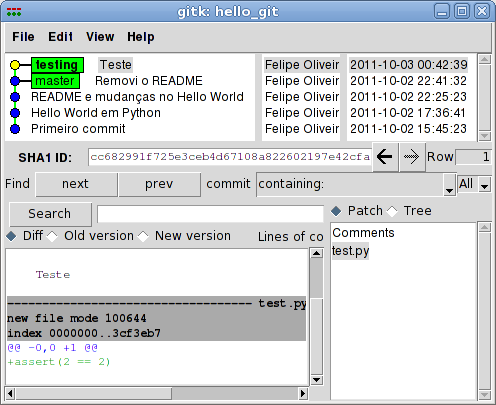
\includegraphics[scale=0.45]{images/gitkhellogittestingbranch.png}
\end{center}
\end{frame}

\begin{frame}[fragile]{Merge simples -- Fast-forward}
\begin{verbatim}
$ git checkout master
Switched to branch 'master'
\end{verbatim}
\pause
\begin{verbatim}
$ git branch
* master
  testing
\end{verbatim}
\pause
\begin{verbatim}
$ git merge testing
Updating b09a767..cc68299
Fast-forward
 test.py |    1 +
 1 files changed, 1 insertions(+), 0 deletions(-)
 create mode 100644 test.py
\end{verbatim}
\end{frame}

\begin{frame}
\begin{center}
  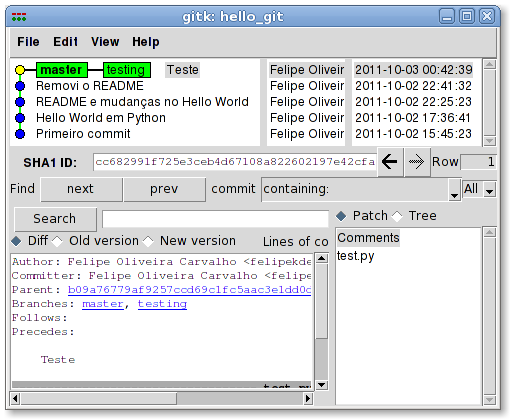
\includegraphics[scale=0.45]{images/gitkhellogitfastforward.png}
\end{center}
\end{frame}

\subsection{Desenvolvimento não-linear}

\begin{frame}{Um exemplo}
\begin{itemize}
  \item Clone o código que está na produção
  \item Crie um branch para issue \#53 (`iss53')
  \item Trabalhe por 10 minutos
  \item Alguém pede um hotfix para a issue \#102
  \item checkout `master'
  \item Crie o branch `iss102'
  \item Resolva o problema
  \item checkout `master`, merge `iss102'
  \item push para a versão pública
  \item checkout `iss53' e continue trabalhando
\end{itemize}
\end{frame}

\begin{frame}{Mais situações}
  \singlephrase{\textbf{Isolar} unidades de trabalho}
\end{frame}

\begin{frame}{Mais situações}
  \singlephrase{Você quer \textbf{experimentar} alguma ideia}
\end{frame}

\begin{frame}{Mais situações}
  \singlephrase{Você vai fazer algo que vai \textbf{demorar}}
\end{frame}

\begin{frame}[fragile]{Passo-a-passo do exemplo}
\begin{center}
Resolva a issue 53. Crie um branch para isso a partir do
\texttt{master}:
\end{center}
\pause
\begin{verbatim}
$ git checkout -b iss53
Switched to a new branch 'iss53'
\end{verbatim}
\pause
\begin{center}
  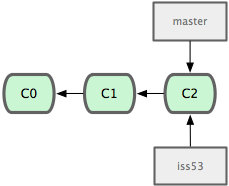
\includegraphics{images/branchiss53.png}
\end{center}
\pause
\begin{center}
Corrija o problema no código:
\end{center}
\begin{verbatim}
$ vim hello_world.py
\end{verbatim}
\end{frame}

\begin{frame}[fragile]{Passo-a-passo do exemplo}
\begin{verbatim}
$ git diff
diff --git a/hello_world.py b/hello_world.py
index ffee107..349aa41 100644
--- a/hello_world.py
+++ b/hello_world.py
@@ -1 +1 @@
-print "Alô mundo!"
+print "Alô, mundo!"
\end{verbatim}
\end{frame}

\begin{frame}[fragile]{Passo-a-passo do exemplo}
\begin{center}
\texttt{commit} das mudanças feitas:
\end{center}
\begin{verbatim}
$ git commit -a -m "Vírgula adicionada [iss53]"
[iss53 63f9671] Vírgula adicionada [iss53]
 1 files changed, 1 insertions(+), 1 deletions(-)
\end{verbatim}
\pause
\begin{center}
  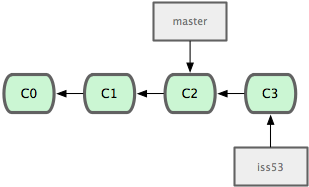
\includegraphics{images/commitiss53.png}
\end{center}
\end{frame}

\begin{frame}[fragile]{Passo-a-passo do exemplo}
\begin{center}
Uma feature tem que ser implementada agora! Faça \texttt{checkout} do
\texttt{master}, pois a nova feature vai ser implementada a partir do código
estável: supostamente o código no \textit{branch} \texttt{master}.
\end{center}
\begin{verbatim}
$ git checkout master
Switched to branch 'master'
\end{verbatim}
\pause
\begin{center}
Crie um novo \textit{branch} -- \texttt{bomdia} -- para implementar a nova
feature:
\end{center}
\begin{verbatim}
$ git checkout -b bomdia
Switched to a new branch 'bomdia'
\end{verbatim}
\pause
\begin{verbatim}
$ vim bom_dia.py
\end{verbatim}
\end{frame}

\begin{frame}[fragile]{Passo-a-passo do exemplo}
\begin{verbatim}
$ git status
# On branch master
# Untracked files:
#   (use "git add <file>..." to include in what will be committed)
#
#       bom_dia.py
nothing added to commit but untracked files present (use "git add" to track)
\end{verbatim}
\pause
\begin{verbatim}
$ git add bom_dia.py
\end{verbatim}
\end{frame}

\begin{frame}[fragile]{Passo-a-passo do exemplo}
\begin{verbatim}
$ git diff --staged
diff --git a/bom_dia.py b/bom_dia.py
new file mode 100644
index 0000000..b62bb76
--- /dev/null
+++ b/bom_dia.py
@@ -0,0 +1 @@
+print "Bom dia!"
\end{verbatim}
\end{frame}

\begin{frame}[fragile]{Passo-a-passo do exemplo}
\begin{center}
\texttt{commit} do "bom dia":
\end{center}
\pause
\begin{verbatim}
$ git commit -a # use o editor para inserir a mensagem
[master cf9146f] Nova feature: script que diz "bom dia"
 1 files changed, 1 insertions(+), 0 deletions(-)
 create mode 100644 bom_dia.py
\end{verbatim}
\pause
\begin{center}
  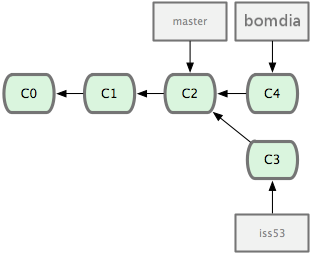
\includegraphics{images/commitbomdia.png}
\end{center}
\end{frame}

\begin{frame}[fragile]{Passo-a-passo do exemplo}
\begin{center}
Adicionando mudanças ao branch \textit{branch} \texttt{master}.
\end{center}
\pause
\begin{verbatim}
$ git checkout master
$ git merge bomdia
Updating cc68299..296d018
Fast-forward
 bom_dia.py |    1 +
 1 files changed, 1 insertions(+), 0 deletions(-)
 create mode 100644 bom_dia.py
\end{verbatim}
\end{frame}

\begin{frame}[fragile]{Passo-a-passo do exemplo}
  \img{images/mergebomdia.png}
\end{frame}

\begin{frame}[fragile]{Passo-a-passo do exemplo}
\begin{center}
O \texttt{merge} já foi feito, então você pode deletar o \textit{branch}
\texttt{bomdia}. \texttt{master} contém o código com a feature que foi
solicitada. Então esse código pode ser enviado para a produção (ou não).
\end{center}
\pause
\begin{verbatim}
$ git branch -d bomdia
Deleted branch bomdia (was 296d018).
\end{verbatim}
\pause
\begin{center}
E agora você pode continuar a trabalhar na resulução da issue \#53.
\end{center}
\pause
\begin{verbatim}
$ git checkout iss53
Switched to branch 'iss53'
\end{verbatim}
\end{frame}

\begin{frame}[fragile]{Passo-a-passo do exemplo}
\pause
\begin{verbatim}
$ vim hello_world.py
$ git commit -a -m "mundo => Mundo"
[iss53 e4c9096] mundo => Mundo
 1 files changed, 1 insertions(+), 1 deletions(-)
\end{verbatim}
\pause
\img{images/secondcommitiss53.png}
\end{frame}

\begin{frame}[fragile]{Passo-a-passo do exemplo}
\begin{center}
\textit{merge} \texttt{iss53} com o \texttt{master}.
\end{center}
\begin{verbatim}
$ git checkout master
Switched to branch 'master'
$ git merge iss53
Merge made by recursive.
 hello_world.py |    2 +-
 1 files changed, 1 insertions(+), 1 deletions(-)
\end{verbatim}
\end{frame}

\begin{frame}{Passo-a-passo do exemplo}
  \img{images/mergeiss53.png}
\end{frame}

\begin{frame}
\begin{center}
  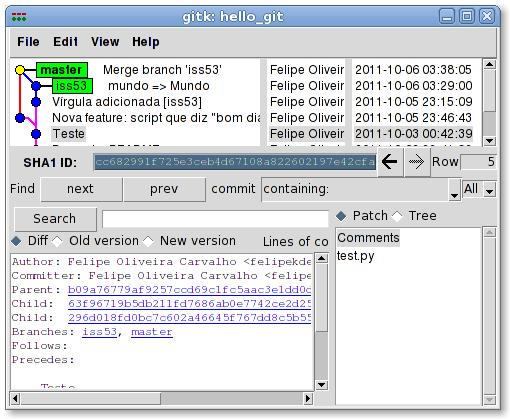
\includegraphics[scale=.38]{images/gitkmergeiss53.png}
\end{center}
\end{frame}

\subsection{Resolvendo conflitos de merge}

\begin{frame}[fragile]
\begin{verbatim}
$ git merge umbranch
Auto-merging hello_world.py
CONFLICT (content): Merge conflict in hello_world.py
Automatic merge failed; fix conflicts and then commit the result.
\end{verbatim}
\pause
\begin{verbatim}
$ cat hello_world.py
<<<<<<< HEAD
print "Alô, Mundo!" # Imprime Alô, Mundo
=======
print "Alô, Mundo!" # LOL
>>>>>>> umbranch
\end{verbatim}
\end{frame}

\section{git no servidor}

\sectiontoc

\subsection{Introdução}

\begin{frame}[fragile]{Criando um projeto no servidor}
\begin{verbatim}
$ git clone --bare my_project my_project.git
Initialized empty Git repository in /opt/projects/my_project.git/
\end{verbatim}
\pause
\begin{verbatim}
$ scp -r my_project.git user@git.example.com:/opt/git
\end{verbatim}
\pause
\begin{center}
Outro usuário clona o repositório
\end{center}
\begin{verbatim}
$ git clone user@git.example.com:/opt/git/my_project.git
\end{verbatim}
\pause
\begin{verbatim}
$ ssh user@git.example.com
$ cd /opt/git/my_project.git
$ git init --bare --shared
\end{verbatim}
\end{frame}

\begin{frame}[fragile]
\begin{center}
Outros usuários podem enviar as mudanças para o repositório no servidor.
\end{center}
\begin{verbatim}
$ vim README
$ git commit -am 'fix for the README file'
$ git push origin master
\end{verbatim}
\end{frame}

\begin{frame}{github}
\begin{center}
\texttt{http://github.com}
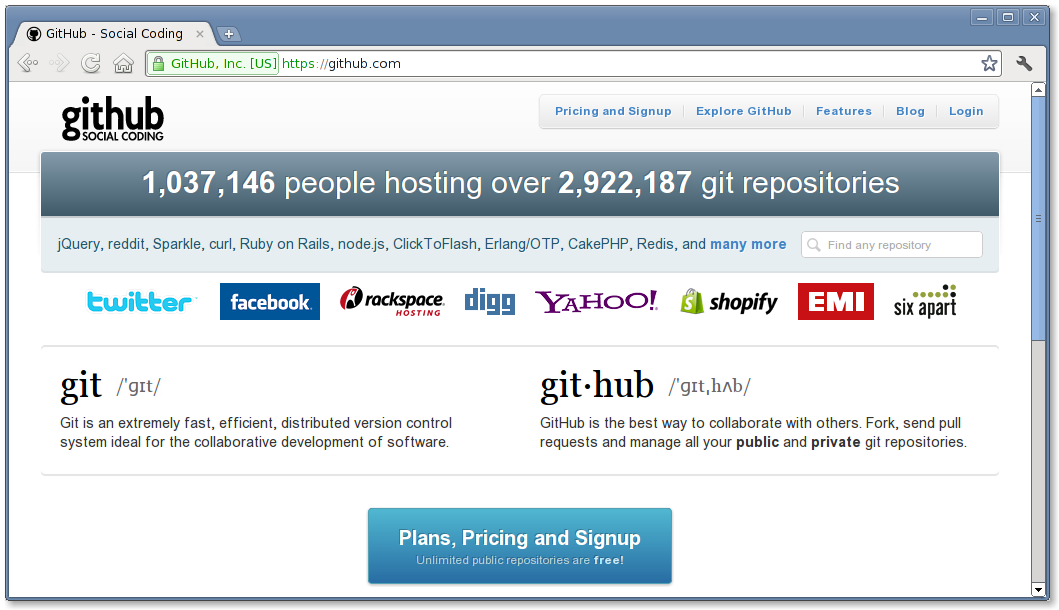
\includegraphics[scale=.3]{images/github.png}
\end{center}
\end{frame}

\subsection{Trabalhando em grupo}

\begin{frame}[fragile]{Workflow básico}
\begin{center}
Usuário clona o repositório remoto com \texttt{git clone} e trabalha localmente.
\end{center}
\pause
\begin{verbatim}
$ vim TODO 
$ git commit -a
\end{verbatim}
\pause
\begin{center}
Usuário quer enviar suas mudanças para o servidor:
\end{center}
\begin{verbatim}
$ git fetch origin
$ git merge origin/master
$ git push
\end{verbatim}
\end{frame}

\begin{frame}{git pull}
  \singlephrase{\texttt{git pull = fetch + merge}}
\end{frame}

\section{Extras}

\begin{frame}{Comandos úteis}
  \begin{itemize}
    \item \texttt{git blame}
    \pause
    \item \texttt{git grep}
    \pause
    \item \texttt{git cherry-pick}
    \pause
    \item \texttt{git stash}
  \end{itemize}
\end{frame}

\begin{frame}[fragile]
  \begin{center}
    \huge \textbf{git stash}
    \item \texttt{save}
    \pause
    \item \texttt{list}
    \pause
    \item \texttt{drop}
    \pause
    \item \texttt{pop}
    \pause
    \item \texttt{apply}
  \end{center}
\end{frame}

\begin{frame}{Pro Git}
\begin{center}
\texttt{http://progit.org}
\end{center}
\begin{center}
  
\includegraphics[scale=.3]{images/progit.jpg}
\end{center}
\end{frame}

\section*{Mais perguntas}

\begin{frame}{Mais perguntas?}
  \singlephrase{Mais perguntas?}
\end{frame}

\end{document}
